\subsection{Interpreting the Second Derivative \& Formal Definition of Concavity}
While the first derivative told us if our function was increasing or decreasing, the
second derivative tells us about concavity!
\begin{Definition}{}{}
    The graph of $ f $ is \textbf{concave upwards} on an interval $ I $ if,
    for every pair of points $ a,b\in I $, the secant line joining
    $ (a,f(a)) $ to $ (b,f(b)) $
    lies above the graph of $ f(x) $.

    The graph is \textbf{concave downwards} on $ I $ if the secant line lies below the graph of $ f $.
\end{Definition}
We can see if the graph is concave up, then the slope of the tangent line is increasing, that is, $ f' $
is increasing. Similarly, if the graph of $ f $ is concave down, then $ f' $ is decreasing. So we get:
\begin{Theorem}{}{}
    \begin{enumerate}[(1)]
        \item If $ f''(x)>0 $ for all $ x\in I $, then the graph of $ f $ is concave up on $ I $.
        \item If $ f''(x)<0 $ for all $ x\in I $, then the graph of $ f $ is concave down on $ I $.
    \end{enumerate}
\end{Theorem}
We also have a name for a point where concavity changes:
\begin{Definition}{}{}
    A point $ c $ is called an \textbf{inflection point} for $ f $ if $ f $
    is continuous at $ x=c $ and the concavity of $ f $ changes at $ x=c $.
\end{Definition}
If $ f''(x) $ is also continuous at $ x=c $, then the sign of $ f'' $ must change at $ x=c $,
so by the IVT, we get:
\begin{Theorem}{}{}
    If $ f''(x) $ is continuous at $ x=c $ and $ (c,f(c)) $ is an inflection point for $ f $,
    then $ f''(c)=0 $.
\end{Theorem}
\begin{Remark}{}{}
    Note that this is only telling us how to find candidates for inflection points. The converse
    is false! If $ f''(c)=0 $, then that does not mean that $ (c,f(c)) $ is an inflection point.
    \begin{Exercise}{}{}
        Find a counterexample!
    \end{Exercise}
\end{Remark}
\begin{Example}{}{}
    Find intervals of concavity and inflection points for $ f(x)=x^4-6x^2 $.
    \tcblower{}
    \textbf{Solution}. $ f'(x)=4x^3-12x $ and $ f''(x)=12x^2-12 $.
    Setting $ f''(x)=0 $ yields $ x=\pm 1 $, let's check:
    \[ \begin{array}{cccc}
                & (-\infty,-1] & (-1,1) & [1,\infty) \\
            f'' & +            & -      & +          \\
            f   & up           & down   & up
        \end{array} \]
    Therefore, $ f $ is concave up on $ (-\infty,-1] $ and $ [1,\infty) $ and concave down on $ [-1,1] $. Since
    $ f'' $ changes at $ x=\pm 1 $ and $ f $ is continuous at $ x=\pm 1 $, these are both inflection points.
\end{Example}
\begin{Example}{}{}
    Find intervals of concavity and inflection points for $ f(x)=\frac{1}{x} $.
    \tcblower{}
    \textbf{Solution}. $ f'(x)=-1/x^2 $, $ f''(x)=2/x^3 $. Note that $ f'' $ is undefined at $ x=0 $.
    \[ \begin{array}{ccc}
                & (-\infty,0) & (0,\infty) \\
            f'' & -           & +          \\
            f   & down        & up
        \end{array} \]
    Therefore, $ f $ is concave up on $ (0,\infty) $ and concave down on $ (-\infty,0) $. However, $ x=0 $
    is \underline{not} an inflection point since $ f $ is continuous at $ x=0 $.
\end{Example}
\subsection{Classifying Critical Points: The First and Second Derivative Tests}
We know that if $ c $ is a local max/min for $ f $, then either $ f'(c)=0 $
or $ f'(c) $ is undefined, that is, $ c $ is a critical point. But not all critical points
are local max/mins! So, let's examine two methods for classifying critical points.
\subsubsection*{Method 1: The First Derivative Test}
\begin{itemize}
    \item Idea: look at the sign of $ f' $ on either side of $ c $.
    \item Say $ f'(x)<0 $ for $ x\in(a,c) $ and $ f'(x)>0 $ for $ x\in(c,b) $ ($ a<c<b $).
    \item Then, $ f $ is decreasing on $ (a,c) $ and increasing on $ (c,b) $. This suggests $ f $
          has a local minimum! Similarly, for local maximums.
\end{itemize}
Let's collect these results into a theorem!
\begin{Theorem}{First Derivative Test}{}
    Assume $ c $ is a critical point for $ f $ and $ f $ is continuous at $ x=c $.
    Let $ c\in (a,b) $.
    \begin{enumerate}[(1)]
        \item $ \bigl(\forall x\in (a,c):f'(x)>0\bigr)\land \bigl(\forall x\in(c,b):f'(x)<0\bigr)
                  \implies f\text{ has a local maximum at }x=c $.
        \item $ \bigl(\forall x\in (a,c):f'(x)<0\bigr)\land \bigl(\forall x\in(c,b):f'(x)>0\bigr)
                  \implies f\text{ has a local minimum at }x=c $.
    \end{enumerate}
\end{Theorem}
These are easier to see if you make a table.
\[ \begin{array}{ccc}
           & (a,c)                           & (c,b)    \\
        f' & +                               & -        \\
        f  & \nearrow                        & \searrow \\
           & \multicolumn{2}{c}{\emph{LMAX}}
    \end{array}\qquad
    \begin{array}{ccc}
           & (a,c)                           & (c,b)    \\
        f' & -                               & +        \\
        f  & \searrow                        & \nearrow \\
           & \multicolumn{2}{c}{\emph{LMIN}}
    \end{array} \]
\begin{Example}{}{}
    Find the local max/mins of $ f(x)=\frac{x^3}{3}-\frac{3x^2}{2}+2x+1 $.
    \tcblower{}
    \textbf{Solution}. $ f'(x)=x^2-3x+2=(x-2)(x-1) $. Hence, $ f'(x)=0 $ when $ x=1 $ and/or $ x=2 $;
    these are both critical points.
    \[ \begin{array}{cccc}
               & (-\infty,1) & (1,2)    & (2,\infty) \\
            f' & +           & -        & +          \\
            f  & \nearrow    & \searrow & \nearrow
        \end{array} \]
    So, $ f $ has a local max at $ x=1 $ and a local min at $ x=2 $ by the first derivative test.
\end{Example}
\subsubsection*{Method 2: The Second Derivative Test}
Suppose $ f'(c)=0 $, so $ c $ is a critical point of $ f $. Then, the tangent line to the
graph of $ f $ at $ x=c $ is horizontal. Suppose also that $ f''(c)<0 $. Then, the tangent line sits
above the graph since the graph is concave down! So, $ x=c $ is a local max! This is the second derivative
test! We get a similar result for $ f''(c)>0 $.
\begin{Theorem}{Second Derivative Test}{}
    Let $ f'(c)=0 $, and let $ f'' $ be continuous at $ x=c $.
    \begin{enumerate}[(1)]
        \item $ f''(c)<0\implies \text{$f$ has a local maximum at $x=c$} $.
        \item $ f''(c)>0\implies \text{$f$ has a local minimum at $x=c$} $.
        \item $ f''(c)=0\implies \text{no information} $.
    \end{enumerate}
\end{Theorem}
\begin{Example}{}{}
    $ f(x)=\frac{x^3}{3}+3x^2-7x+3 $.
    \tcblower{}
    \textbf{Solution}. $ f'(x)=x^2+6x-7=(x-1)(x+7) $. Hence, $ f'(x)=0 $ when $ x=-7 $ and/or $ x=1 $.
    Note that $ f''(x)=2x+6 $ is continuous on $ \R $.
    \begin{itemize}
        \item $ f''(-7)=-8<0 \implies x=-7 $ is a local maximum.
        \item $ f''(1)=8>0 \implies x=1 $ is a local minimum.
    \end{itemize}
\end{Example}
\begin{Remark}{}{}
    You can use either the first or second derivative test to classify critical points, whichever you prefer!
\end{Remark}
\section{Curve Sketching}
To sketch $ f(x) $:
\begin{enumerate}[(1)]
    \item Find the domain of $ f $.
    \item Find all the intercepts ($ x $-int ($ y=0 $) and $ y $-int ($ x=0 $)).
    \item \begin{enumerate}[(a)]
              \item Find all vertical asymptotes ($ \div 0 $, $ \ln $)
              \item Find all horizontal asymptotes ($ \lim\limits_{{x} \to {\pm\infty}}f(x) $).
          \end{enumerate}
    \item Find $ f'(x) $ and any critical points ($ (x,y) $ coordinates).
    \item Find $ f''(x) $ and solve $ f''(x)=0 $, find any points where $ f''(x) $ does not exist ($ (x,y) $ coordinates).
    \item Test all intervals for increasing/decreasing, concavity, inflection points, local extrema.
    \item Plot the interest points and asymptotes on a graph.
    \item Connect the dots using the following:
          \[ \begin{array}{ccc}
                       & f''>0                                                      & f''<0                                                     \\
                  f'>0 & \tikz[scale=0.5]{\draw[-] (0,0) to [bend right=50] (1,1)}  & \tikz[scale=0.5]{\draw[-] (0,0) to [bend left=50] (1,1)}  \\
                  f'<0 & \tikz[scale=0.5]{\draw[-] (0,0) to [bend right=50] (1,-1)} & \tikz[scale=0.5]{\draw[-] (0,0) to [bend left=50] (1,-1)}
              \end{array} \]
\end{enumerate}
\begin{Example}{}{}
    Sketch $ f(x)=x^4-16x^2 $ with calculus.
    \tcblower{}
    \textbf{Solution}.
    \begin{enumerate}[(1)]
        \item Domain: $ \R $.
        \item \begin{itemize}
                  \item $ x $-int ($ y=0 $): $ 0=x^4-16x^2=x^2(x-4)(x+4)\implies x=0,\pm 4 $. Points: $ (0,0) $, $ (4,0) $, $ (-4,0) $.
                  \item $ y $-int ($ x=0 $): $ (0,0) $.
              \end{itemize}
        \item No VA's, no HA's.
        \item $ f'(x)=4x^3-32x=4x(x-\sqrt{8})(x+\sqrt{8})=0 $ if $ x=0,\pm\sqrt{8} $ (all critical points).
        \item $ f''(x)=12x^2-32=4(3x^2-8)=0 $ if $ x=\pm\sqrt{\tfrac{8}{3}} $. Points: $ (\pm\sqrt{\tfrac{8}{3}},-\tfrac{320}{9}) $.
        \item The test:
              \[ \begin{NiceArray}{|c|c|c|c|c|c|c|}
                      \toprule
                                   & (-\infty,-\sqrt{8})                                        & (-\sqrt{8},-\sqrt{\tfrac{8}{3}})                          & (-\sqrt{\tfrac{8}{3}},0)                                 & (0,\sqrt{\tfrac{8}{3}})                                   & (\sqrt{\tfrac{8}{3}},\sqrt{8})                             & (\sqrt{8},\infty)                                         \\
                      \midrule
                      f''          & \multicolumn{2}{c}{+}                                      & \multicolumn{2}{c}{-}                                     & \multicolumn{2}{c}{+}                                                                                                                                                                                                                         \\
                      \midrule
                      f'           & -                                                          & \multicolumn{2}{c}{+}                                     & \multicolumn{2}{c}{-}                                    & +                                                                                                                                                                                  \\
                      \midrule
                      f            & \searrow                                                   & \nearrow                                                  & \nearrow                                                 & \searrow                                                  & \searrow                                                   & \nearrow                                                  \\
                      \midrule
                      \text{Shape} & \tikz[scale=0.5]{\draw[-] (0,0) to [bend right=50] (1,-1)} & \tikz[scale=0.5]{\draw[-] (0,0) to [bend right=50] (1,1)} & \tikz[scale=0.5]{\draw[-] (0,0) to [bend left=50] (1,1)} & \tikz[scale=0.5]{\draw[-] (0,0) to [bend left=50] (1,-1)} & \tikz[scale=0.5]{\draw[-] (0,0) to [bend right=50] (1,-1)} & \tikz[scale=0.5]{\draw[-] (0,0) to [bend right=50] (1,1)} \\
                      \bottomrule
                  \end{NiceArray} \]
              It is clear that the local minima are at $ x=\pm\sqrt{8} $ and the local maximum is at $ x=0 $.
    \end{enumerate}
    \begin{center}
        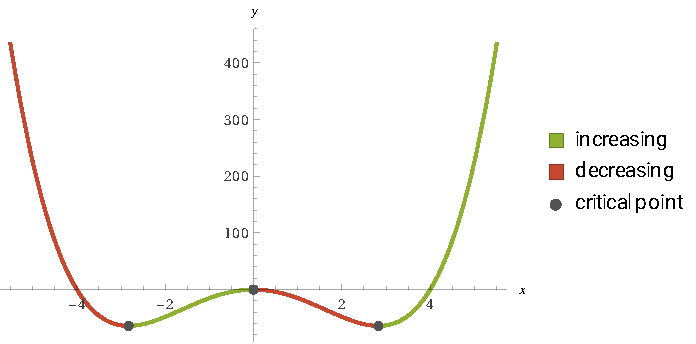
\includegraphics[width=0.48\textwidth]{sketch1.pdf}
        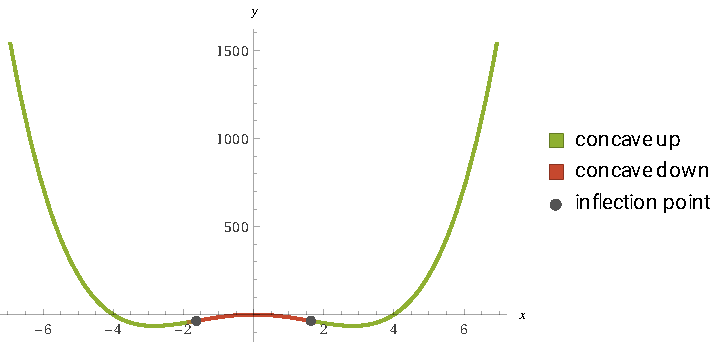
\includegraphics[width=0.48\textwidth]{sketch12.pdf}
    \end{center}
    Hence, $ f $ is:
    \begin{itemize}
        \item Increasing on $ (-\sqrt{8},0) $ and $ (\sqrt{8},\infty) $;
        \item Decreasing on $ (-\infty,-\sqrt{8}) $ and $ (0,\sqrt{8}) $;
        \item Concave up on $ (-\infty,-\sqrt{\tfrac{8}{3}}) $ and $ (\sqrt{\tfrac{8}{3}},\infty) $;
        \item Concave down on $ (-\sqrt{\tfrac{8}{3}},\sqrt{\tfrac{8}{3}}) $.
    \end{itemize}
\end{Example}

\begin{Example}{}{}
    Sketch $ f(x)=e^{-x^2} $ with calculus.
    \tcblower{}
    \textbf{Solution}.
    \begin{enumerate}[(1)]
        \item Domain: $ \R $.
        \item $ y $-int ($ x=0 $): $ y=1 $; no $x$-int.
        \item No VA's.
              \[ \lim\limits_{{x} \to {\pm\infty}}e^{-x^2}=0, \]
              so HA at $ y=0 $ for $ x\to\pm\infty $.
        \item $ f'(x)=e^{-x^2}(-2x)=0 $ if $ x=0 $. Point is $ (0,1) $.
        \item $ f''(x)=-2e^{-x^2}+e^{-x^2}(4x^2)=e^{-x^2}(4x^2-2)=0 $ if $ x=\pm \tfrac{1}{\sqrt{2}} $. Points: $ (\pm \tfrac{1}{\sqrt{2}},\tfrac{1}{\sqrt{e}}) $.
        \item The test:
              \[ \begin{NiceArray}{|c|c|c|c|c|c|c|}
                      \toprule
                                   & (-\infty,-\tfrac{1}{\sqrt{2}})                            & (-\tfrac{1}{\sqrt{2}},0)                                 & (0,\tfrac{1}{\sqrt{2}})                                   & (\tfrac{1}{\sqrt{2}},\infty)                               \\
                      \midrule
                      f''          & +                                                         & \multicolumn{2}{c}{-}                                    & +                                                                                                                      \\
                      \midrule
                      f'           & \multicolumn{2}{c}{+}                                     & \multicolumn{2}{c}{-}                                                                                                                                                             \\
                      \midrule
                      f            & \nearrow                                                  & \nearrow                                                 & \searrow                                                  & \nearrow                                                   \\
                      \midrule
                      \text{Shape} & \tikz[scale=0.5]{\draw[-] (0,0) to [bend right=50] (1,1)} & \tikz[scale=0.5]{\draw[-] (0,0) to [bend left=50] (1,1)} & \tikz[scale=0.5]{\draw[-] (0,0) to [bend left=50] (1,-1)} & \tikz[scale=0.5]{\draw[-] (0,0) to [bend right=50] (1,-1)} \\
                      \bottomrule
                  \end{NiceArray} \]
              It is clear that the local maximum is at $ x=0 $.
    \end{enumerate}
    \begin{center}
        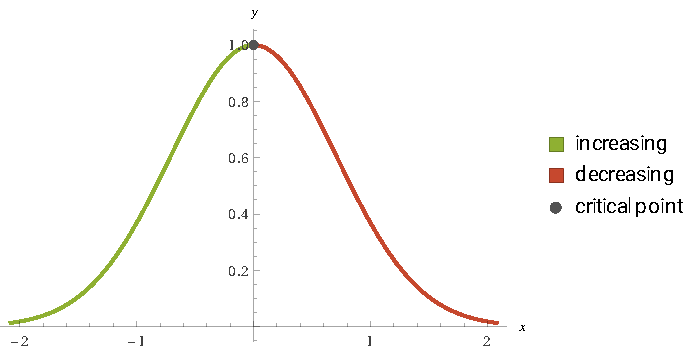
\includegraphics[width=0.48\textwidth]{sketch2.pdf}
        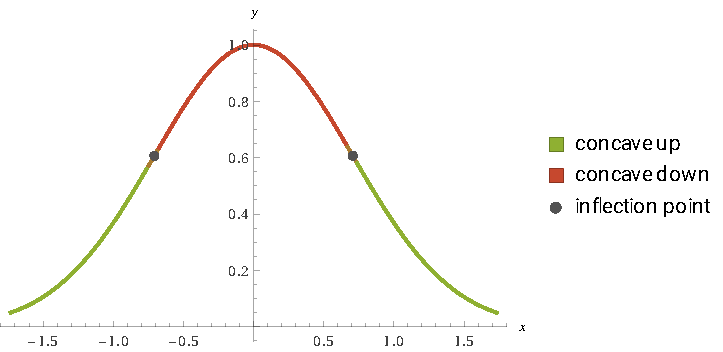
\includegraphics[width=0.48\textwidth]{sketch22.pdf}
    \end{center}
    Hence, $ f $ is:
    \begin{itemize}
        \item Increasing on $ (-\infty,0) $;
        \item Decreasing on $ (0,\infty) $;
        \item Concave up on $ (-\infty,-\tfrac{1}{\sqrt{2}}) $ and $ (\tfrac{1}{\sqrt{2}},\infty) $;
        \item Concave down on $ (-\tfrac{1}{\sqrt{2}},\tfrac{1}{\sqrt{2}}) $.
    \end{itemize}
\end{Example}
\begin{Example}{}{}
    Sketch $ \displaystyle f(x)=\frac{x^2}{x^2-4} $ with calculus. Note that
    \[ f'(x)=-\frac{8x}{(x^2-4)^2},\quad f''(x)=\frac{8(3x^2+4)}{(x^2-4)^3}. \]
    \tcblower{}
    \textbf{Solution}.
    \begin{enumerate}[(1)]
        \item Domain: $ x\ne \pm 2 $.
        \item $x$ and $ y $-int ($ x=0 $, $y=0$): $ (0,0) $
        \item VA at $ x=\pm 2 $.
              \[ \lim\limits_{{x} \to {\pm\infty}}f(x)=1, \]
              so HA at $ y=1 $ for $ x\to\pm\infty $.
        \item $ f'(x)=0 $ when $ x=0 $. $ f'(x) $ DNE if $ x=\pm 2 $, but $ x=\pm 2 $ is not in the domain of the function. Therefore, the only critical point is $ x=0 $.
        \item $ f''(x)=0 $ never. $ f''(x) $ DNE when $ x=\pm 2 $.
        \item The test:
              \[ \begin{NiceArray}{|c|c|c|c|c|c|c|}
                      \toprule
                                   & (-\infty,-2)                                              & (-2,0)                                                   & (0,2)                                                     & (2,\infty)                                                 \\
                      \midrule
                      f''          & +                                                         & \multicolumn{2}{c}{-}                                    & +                                                                                                                      \\
                      \midrule
                      f'           & +                                                         & +                                                        & -                                                         & -                                                          \\
                      \midrule
                      f            & \nearrow                                                  & \nearrow                                                 & \searrow                                                  & \searrow                                                   \\
                      \midrule
                      \text{Shape} & \tikz[scale=0.5]{\draw[-] (0,0) to [bend right=50] (1,1)} & \tikz[scale=0.5]{\draw[-] (0,0) to [bend left=50] (1,1)} & \tikz[scale=0.5]{\draw[-] (0,0) to [bend left=50] (1,-1)} & \tikz[scale=0.5]{\draw[-] (0,0) to [bend right=50] (1,-1)} \\
                      \bottomrule
                  \end{NiceArray} \]
              It is clear that the local maximum is at $ x=0 $.
    \end{enumerate}
    \begin{center}
        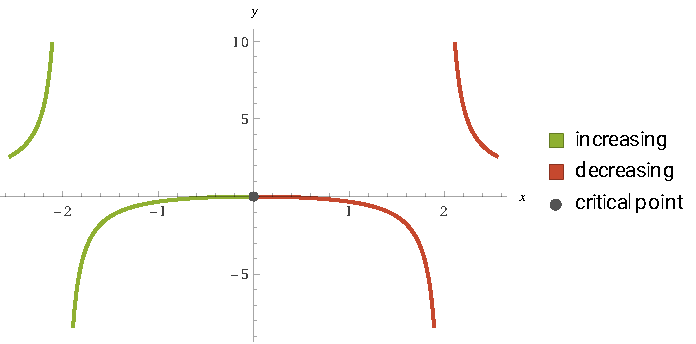
\includegraphics[width=\textwidth]{sketch32.pdf}
    \end{center}
    Hence, $ f $ is:
    \begin{itemize}
        \item Increasing on $ (-\infty,-2) $ and $ (-2,0) $;
        \item Decreasing on $ (0,2) $ and $ (2,\infty) $;
        \item Concave up on $ (-\infty,-2) $ and $ (2,\infty) $;
        \item Concave down on $ (-2,2) $.
    \end{itemize}
\end{Example}